\documentclass[10pt,twocolumn,letterpaper]{article}

\usepackage{cvpr}
\usepackage{times}
\usepackage{epsfig}
\usepackage{graphicx}
\usepackage{amsmath}
\usepackage{amssymb}
% \usepackage{natbib}
\usepackage{subcaption}

% Include other packages here, before hyperref.

% If you comment hyperref and then uncomment it, you should delete
% egpaper.aux before re-running latex.  (Or just hit 'q' on the first latex
% run, let it finish, and you should be clear).
\usepackage[pagebackref=true,breaklinks=true,letterpaper=true,colorlinks,bookmarks=false]{hyperref}
\newcommand{\matr}[1]{\mathbf{#1}} % undergraduate algebra version

\cvprfinalcopy % *** Uncomment this line for the final submission

\def\cvprPaperID{0001} % *** Enter the 3DV Paper ID here
\def\httilde{\mbox{\tt\raisebox{-.5ex}{\symbol{126}}}}

% Pages are numbered in submission mode, and unnumbered in camera-ready
%\ifcvprfinal\pagestyle{empty}\fi
%\setcounter{page}{4321}
\begin{document}

%%%%%%%%% TITLE
\title{Registering Point Clouds to OSM Building Outlines}

\author{Anurag Sai Vempati\\
Autonomus Systems Lab\\ ETH Zurich\\
{\tt\small avempati@ethz.ch}
% For a paper whose authors are all at the same institution,
% omit the following lines up until the closing ``}''.
% Additional authors and addresses can be added with ``\and'',
% just like the second author.
% To save space, use either the email address or home page, not both
\and
Wolf Vollprecht\\
\\ ETH Zurich
\\
{\tt\small wolfv@student.ethz.ch}
}

\maketitle
%\thispagestyle{empty}

%%%%%%%%% ABSTRACT
\begin{abstract}
  The project aims to map point cloud data of outdoor city environments to OpenStreetMaps\footnote{\url{http://www.openstreetmap.org/}} (OSM) building outlines, manually mapped by humans. The point cloud data is generated by using the Structure-from-Motion technique to extract 3D data from multiple photographs taken from different viewpoints. The photographs are taken by consumer grade cameras and processed by software like Bundler ~\cite{snavely2006photo} or VisualSFM ~\cite{visualsfm2011visual}. While point clouds are easy to obtain through processes such as Structure-From-Motion they only exist in a space for themselves. GPS coordinates, recorded at capture time of the images, can give a sparse and noisy reference to the true position of the point cloud. In this paper we present a method to register a point cloud on reference map data thus helping to bridge the gap between two different representations.
\end{abstract}

%%%%%%%%% BODY TEXT
\section{Introduction}

Reconstruction of cityscapes is a well-researched field. Merging OSM data with point clouds and aligning them has been done by Untzelmann et al. \cite{6755957} for the purpose of generating 3D representations of buildings. An indepth approach to georegistration of SfM point clouds was described by Wang~\cite{wang2013accurate}. Strecha~\cite{EPFL-CONF-148247} has shown how large scale city reconstruction from many photographs can be efficiently implemented, using the available metadata, as well as fitting the pointcloud on map data. Reconstruction of abstract building geometry (including roof shape) on basis of aerial \textsc{Lidar} data has been done by Verma~\cite{verma20063d}. The 3D reconstruction of roof shapes by evaluating satellite imagery was demonstrated by Blair~\cite{blair2012towards}. Usually many available images available online are localized highly around major landmarks and thus SfM can only generate partial city landscape. ~\cite{wang2013accurate} have used accurate GPS tagged images from Google Street View to solve this problem. The GPS tags also help in initialization of ICP problem. ~\cite{grzeszczuk2009creating} also performed iterative refinement of the SfM structure after aligning with the building outlines. This helps in removing any imperfections of the SfM pipeline and inaccurate Bundle Adjustment.

  % With current state of  the art technology, obtaining point clouds through structure from motion has become an easy task. 
  % Several attempts deal with a similar problem, such as ... 

\section{Segmenting the Point Cloud and generating 2D outline}

Point clouds that we will be operating on are obtained through Structure from Motion (SfM) techniques. SfM techniques generate 3D structure from a sequence of 2D images that can either be manually taken or collected from online images warehouses like Google images, Flikr etc. We will be using one such software called Bundler\footnote{\url{http://www.cs.cornell.edu/~snavely/bundler/}}. Bundler does incremental reconstruction using Sparse Bundle Adjustment. It updates the structure as additional images are available, eliminating the need to wait for the system to generate structure from scratch which might take several hours. We used the Aachen dataset ~\cite{sattler2012image} containing point cloud generated by bundler using 4479 images taken with different consumer cameras.

For getting a 2D outline of the buildings, we need to be able to segment out the point clouds into parts that belong to a plane which is up-right (and hence shows up as a line in the 2-D map) and the parts that are outliers to these planes. It's also helpful to get rid of noisy points in the point cloud to eliminate drifts and errors further down the pipeline (corner detection, ICP etc.). 

\subsection{Bundler Parser}
The aachen.out file is the output generated by Bundler after registering all the images. It contains the camera calibration for every one of the 4479 images. Bundler file consists of the estimated scene geometry and has the following format\footnote{\url{http://phototour.cs.washington.edu/bundler/bundler-v0.4-manual.html\#S6}}:

{\scriptsize
\begin{verbatim}
    # Bundle file v0.3
    <num_cameras> <num_points>   [two integers]
    <camera1>
    <camera2>
       ...
    <cameraN>
    <point1>
    <point2>
       ...
    <pointM>
\end{verbatim}
}

Each camera entry $<$cameraI$>$ contains camera intrinsics and extrinsics int he following form:

{\scriptsize
\begin{verbatim}
    <f> <k1> <k2>   [focal length, followed by distortion coeffs]
    <R>             [camera rotation]
    <t>             [camera translation]
\end{verbatim}
}

Each point entry $<$pointJ$>$ has the following form:

{\scriptsize
\begin{verbatim}
    <position>      [3D position of the point]
    <color>         [RGB color of the point]
    <view list>     [a list of views the point is visible in]
\end{verbatim}
}

A parser is written that can efficiently read the aachen.out file and store a part or the whole structure into a point cloud (along with RGB color attributes) that can be processed using point cloud library (PCL\footnote{\url{http://www.pointclouds.org/}}). We also store the camera locations $\textbf{c} = -R^{'}t$ for estimating the ground plane.

\subsection{Ground Plane and Point normal estimation}
To be able to generate building 2D outlines, we first estimated the up-vector which is coplanar with the facades of the building and is normal to the ground. Our approach is based on the assumption that majority of the images are taken from ground level and thus fitting a plane through all the camera centers $\textbf{c}$ should be a reasonable estimate of the ground plane. The smallest eigen vector of covariance matrix generated from camera positions is chosen as the up-vector. Fig~\ref{fig:ground} shows the camera positions and the estimated ground plane.

\begin{figure}[h]
   \centering
   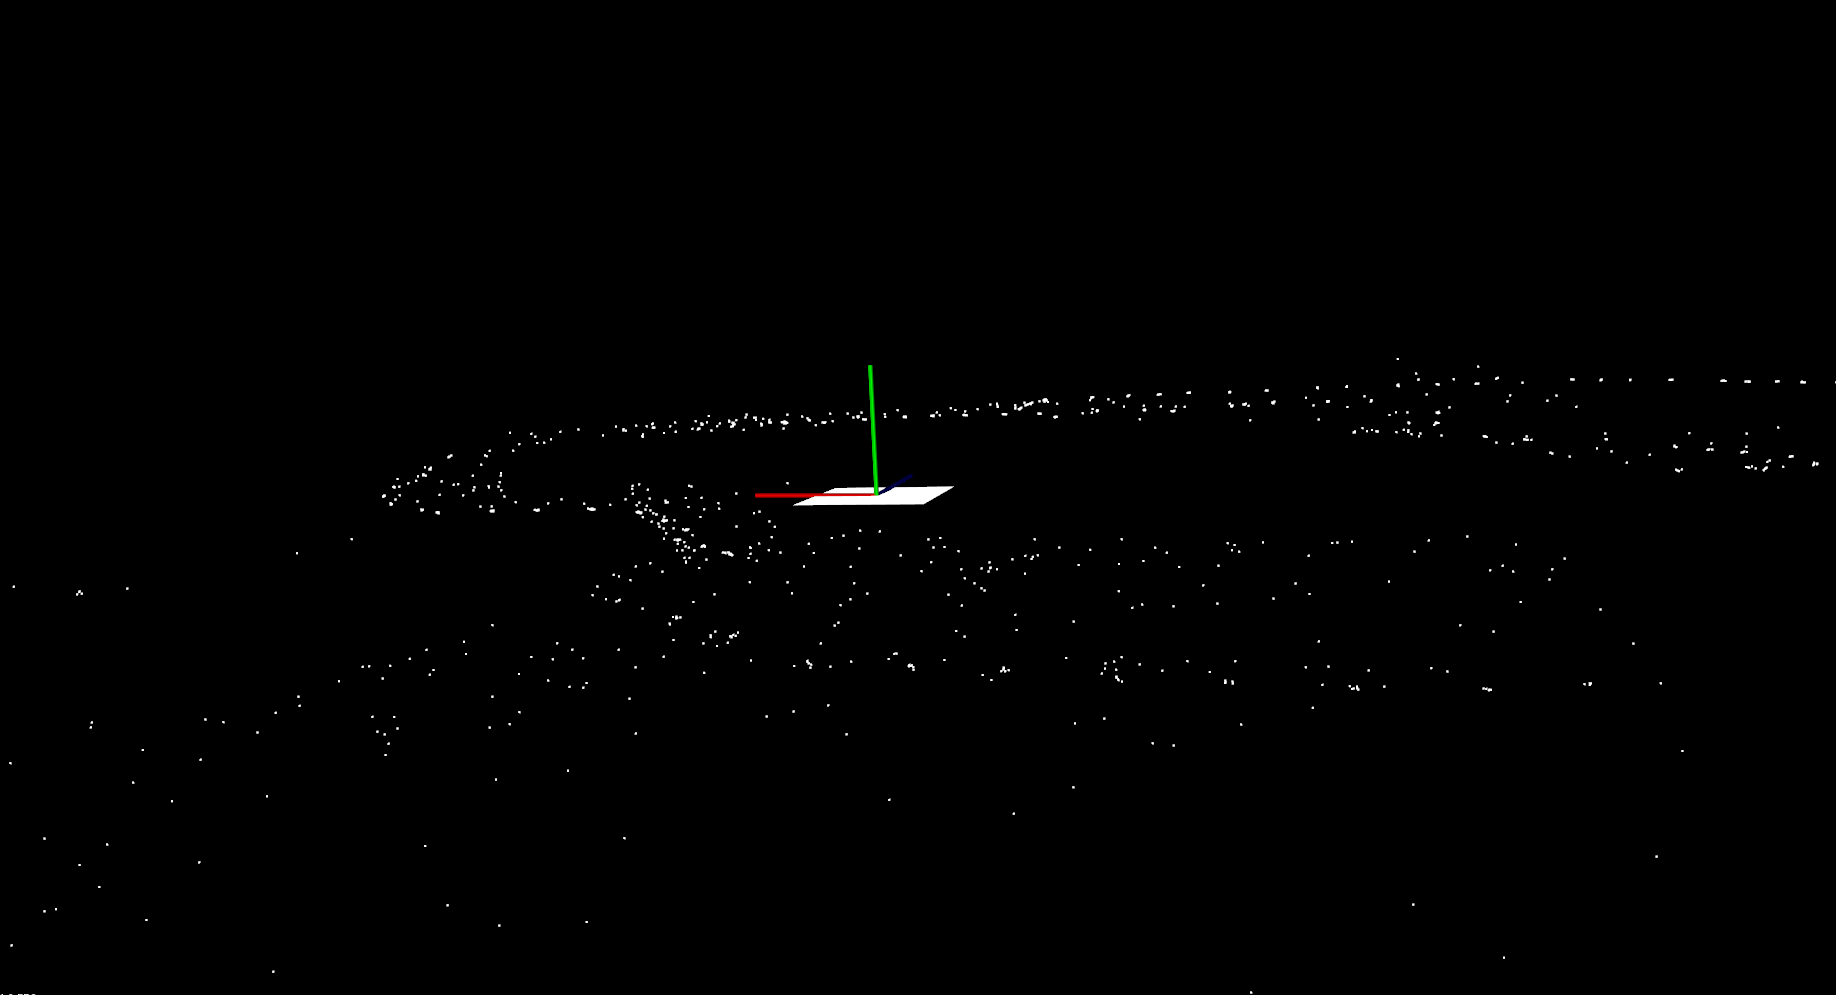
\includegraphics[width=\linewidth]{images/ground_plane.png}
   \caption{Camera positions and estimated ground plane}
   \label{fig:ground}
\end{figure}

The point normals are required to distinguish points that belong to the building facades and the rest. It also helps to filter out the noisy points from the point cloud. point normals are estimated in a similar fashion as the up-vector by evaluating smallest eigen vector of the covariance matrix generated from $\textit{k}$ nearest neighbors of each point in the point cloud. Fig~\ref{fig:normals} shows point normals of a section of the point cloud.

\begin{figure}[h]
   \centering
   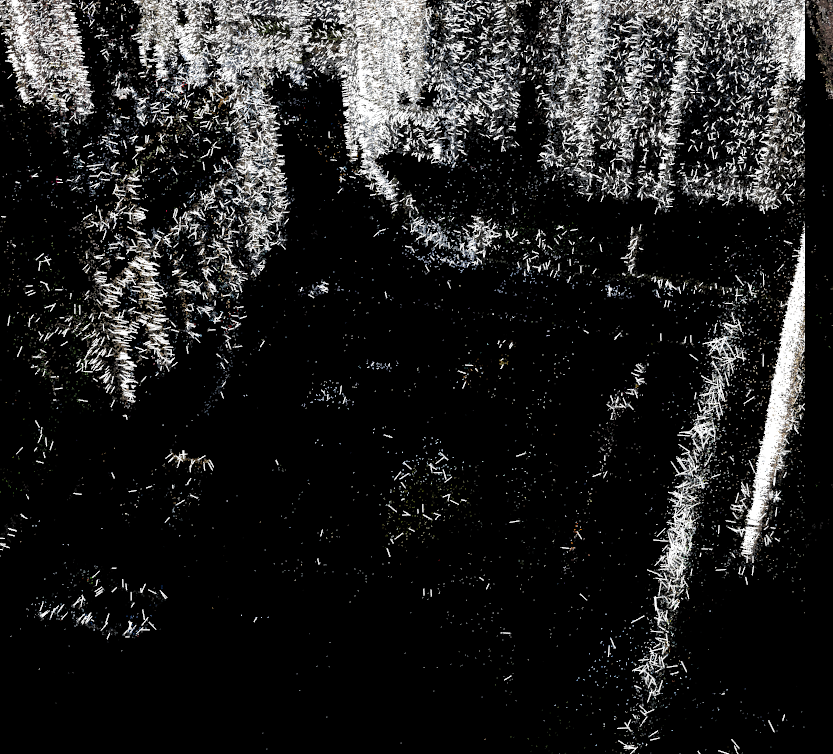
\includegraphics[width=\linewidth]{images/point_normals.png}
   \caption{Point normals}
   \label{fig:normals}
\end{figure}

\subsection{Segmenting the point cloud}
With the knowledge of the ground plane (up-vector) we can calculate the probability for a given point to be on a vertical plane, which makes it a candidate for being part of a facade. Projecting these points onto a ground plane should give us a 2D footprint of the building, similar to what is manually drawn in OSM. This probability $P_{i}$ for each point $i$ is estimated as $\alpha \ 1 - \textit{Dot}(point\_normal_i, up\_vector)$, where $\textit{Dot}(.)$ indicates vector dot product. The point $i$ is assumed to be belonging to a facade if $P_{i} > threshold$. Fig~\ref{fig:seg_cloud} shows the input point cloud (on the left) and the one obtained after segmenting out points belonging to facades (on the right).

\begin{figure}[h]
   \centering
   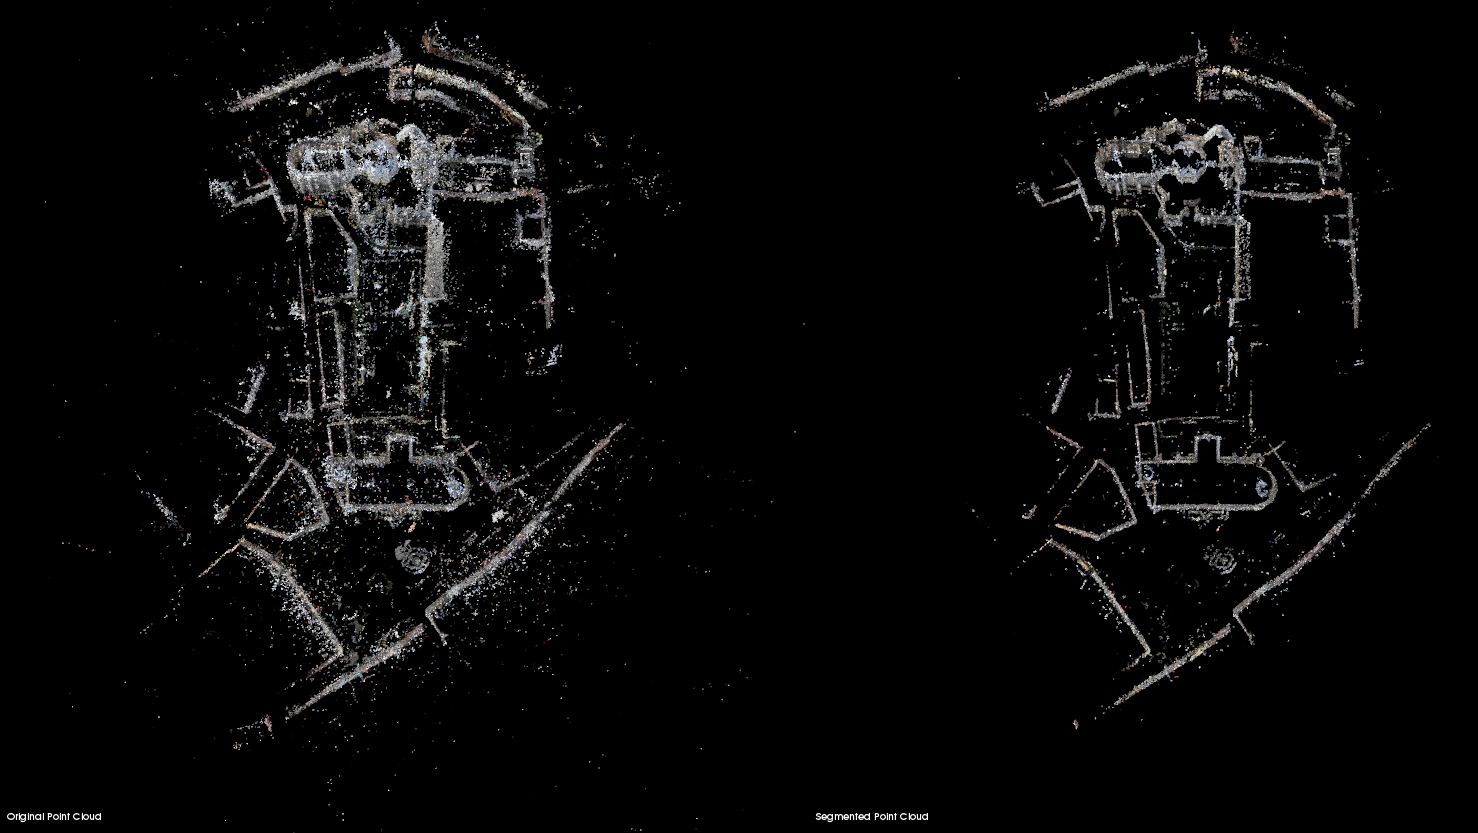
\includegraphics[width=\linewidth]{images/pcl_segmentation.png}
   \caption{Segmented Point Cloud}
   \label{fig:seg_cloud}
\end{figure}

The points of the segmented cloud (on bottom right) are now down-projected onto the ground plane to get a 2D outline (on top) indicating the building footprint as shown in Fig~\ref{fig:pcl_outline}

\begin{figure}[h]
   \centering
   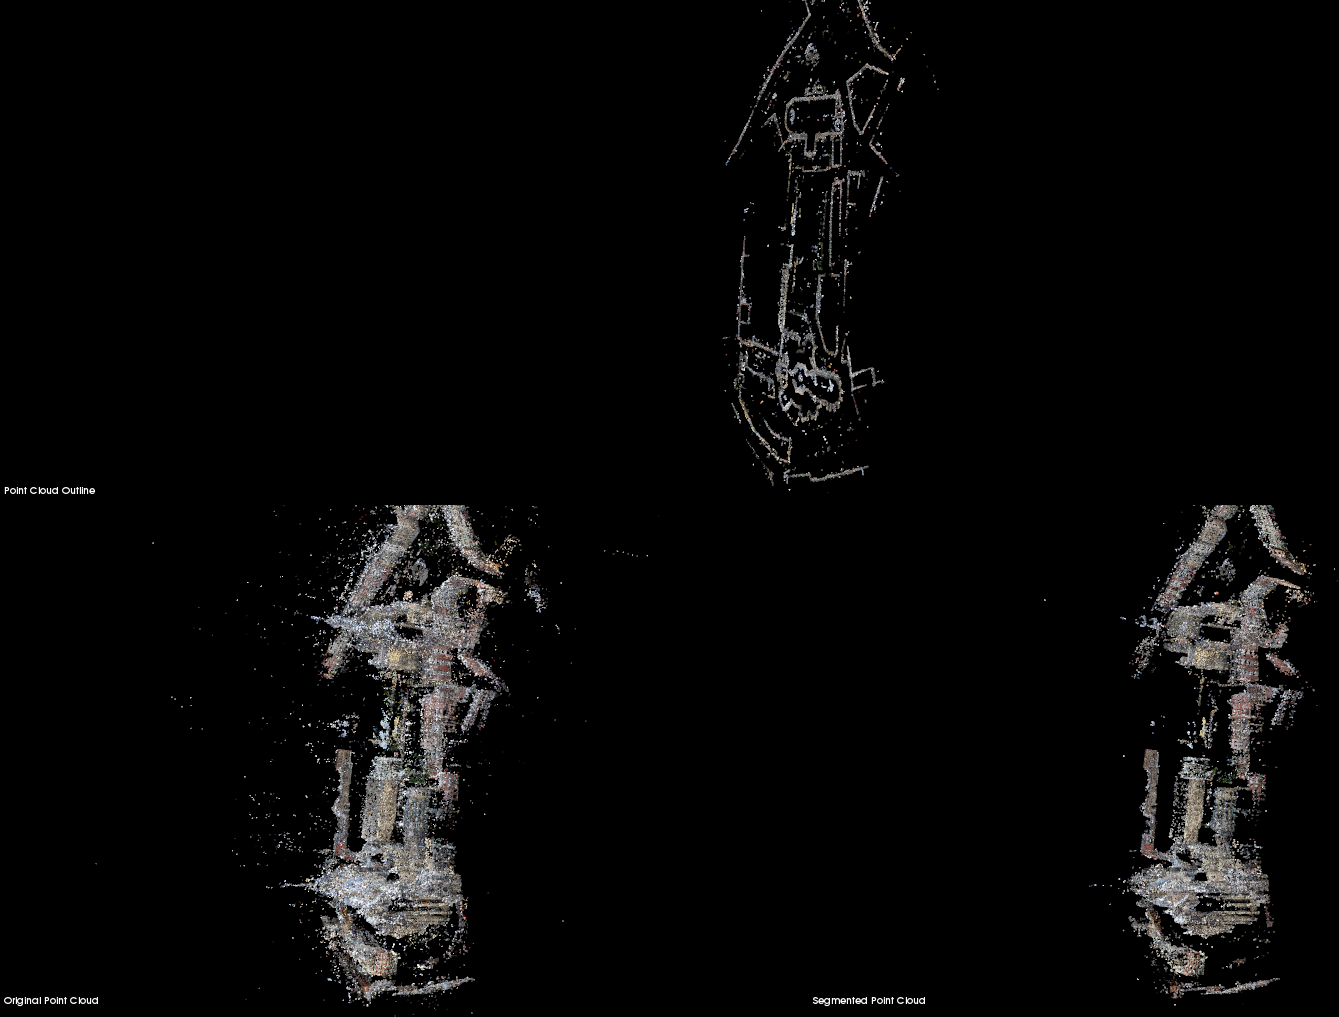
\includegraphics[width=\linewidth]{images/pcl_outline.png}
   \caption{Building footprint obtained from point cloud}
   \label{fig:pcl_outline}
\end{figure}

\section{Obtaining the ground truth}

\begin{figure}[h]
   \centering
   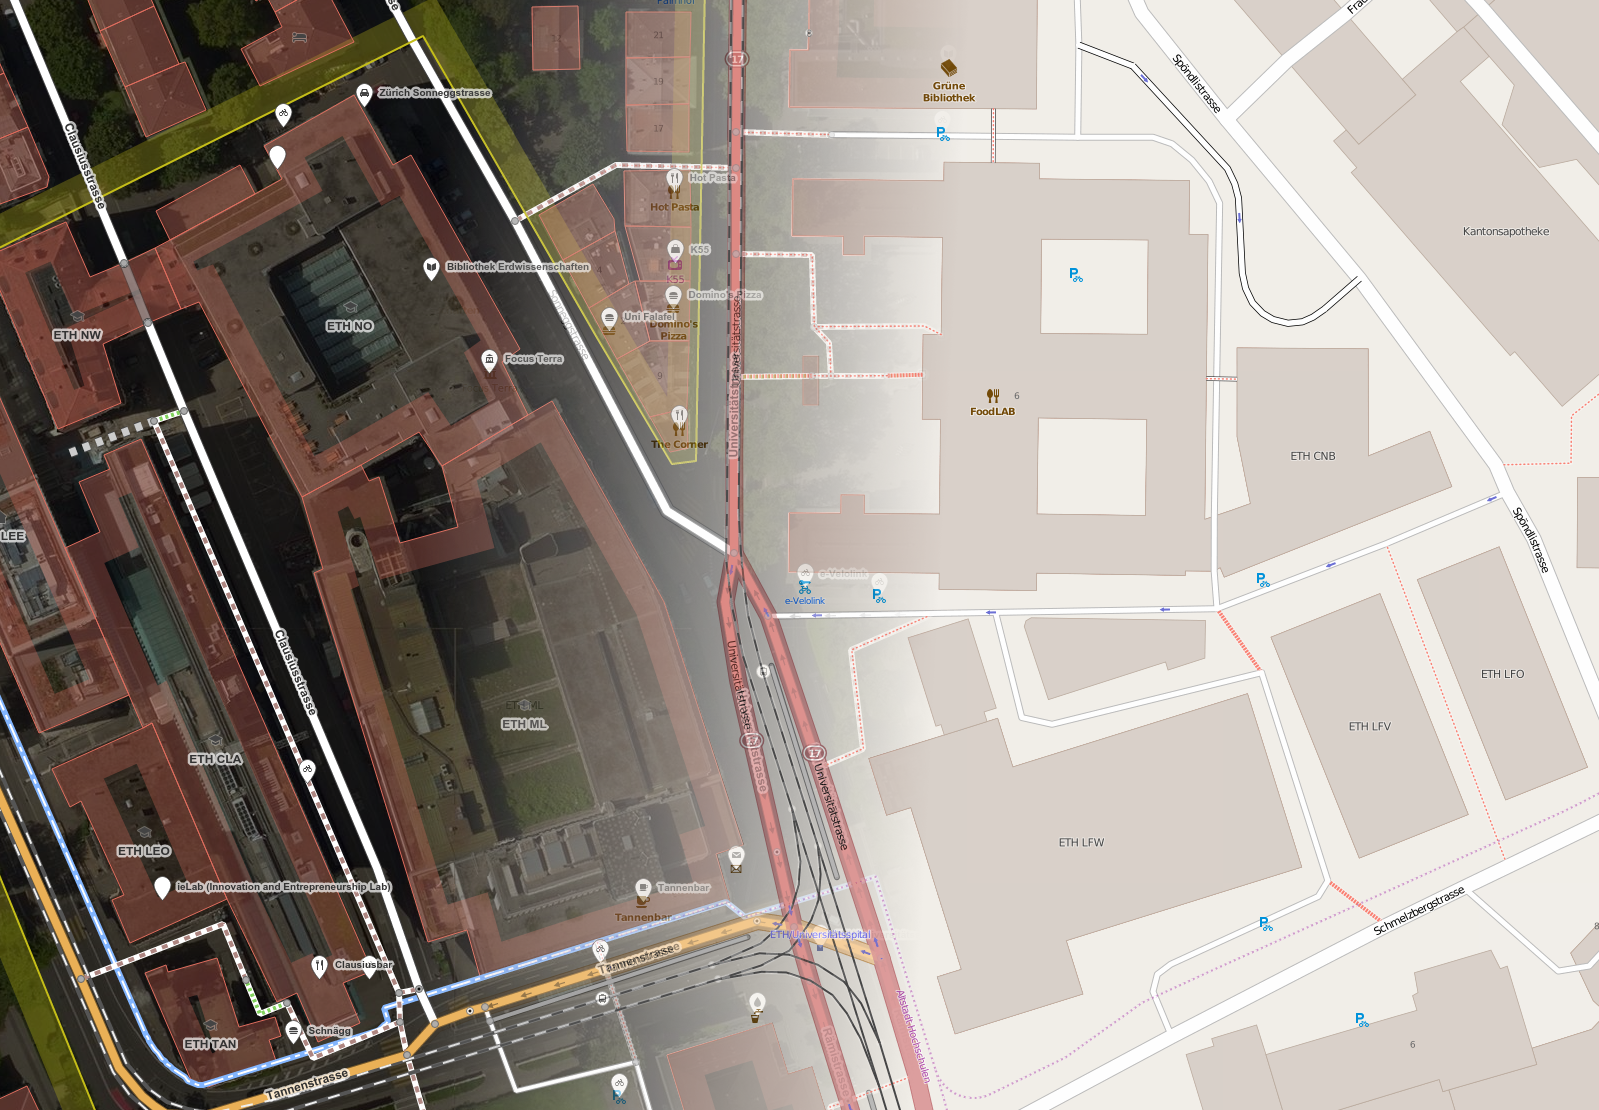
\includegraphics[width=\linewidth]{images/osm_map.png}
   \caption{OSM overlaid with editor interface}
   \label{fig:figure1}
\end{figure}

In order to obtain the ground truth building outlines, we used OpenStreetMaps, a collaborative mapping effort that takes place globally. Volunteers are mapping their surroundings and upload it to a central database, where all changes to the map are stored. 
Of concern for us is only one mapped entity, the building. All points in OSM are stored as nodes. The entity consists of one or more node (in the case of a building it's multiple nodes). By parsing the XML response and mapping all node values to the corresponding building entity, we can obtain all corner points of the closed polygon that describes a building outline in the real world.

In order to adjust the point cloud to the obtained ground truth, we discretized the polygons to point clouds themselves by creating points along the polygon edges in a certain distance. During the Iterative Closest Point matching these points will be matched against the point cloud and provide an error distance.

The OSM data is in the standard latitude/longitude coordinate format. This representation maps coordinates to the globe, which has a spherical shape. However, we would like to work on a 2D surface. The size of the registration is reasonably small to obtain a 2D representation that falls into the boundaries of acceptable error.

There are a number of methods on how to convert coordinates to a 2D representation, which is a topic that has been explored for a long time since large-scale mapping has taken place globally. An exhaustive overview can be found in Snyder (1987)~\cite{Snyder1987}. The methods can be divided into two different categories:

\begin{itemize}
   \item \textbf{Conformal} This category of mappings preserves angles as observed in the real world (i.e. the local angles are preserved). 
   \item \textbf{Equiareal} Retains equal area
   \item \textbf{Equidistant} Preserving distance
   \item \textbf{Azimuthal} Preserving Direction
   \item \textbf{Shortest Route} Shortest route is observable 
\end{itemize}

Since the sphere cannot be flattened out without distortion (ie. the sphere is a non-developable surface) not all of the above properties can hold for a projection at the same time.

For our application of registering a 2D point cloud on the map, we chose to use the Universal Transverse Mercator (UTM) projection, which preserves the angles and shapes, a property we deemed useful for our application.

Contrary to other map projections, UTM is not a single projection but rather divides the globe into 60 different zones.

\section{Registering the Point Cloud}

After obtaining the ground truth and the 2D projection of the 3D cloud we are now able to register the point cloud on the OSM reference.

Therefore we use ``Iterative Closest Point'' (ICP) matching algorithm. As the name suggest, ICP is an iterative algorithm to minimize the distance between two (or more) point cloud measurements. ICP is a widely used algorithm for example in robotics (Simultaneous Localization and Mapping [SLAM]). 

The input to the ICP algorithm in general is two pointclouds, one called the reference and the other source. The source should be aligned to the reference cloud. The output of the algorithm is a transformation matrix in 2 or 3 dimensions. Furthermore, the algorithm needs to be supplied with a stop condition, for example a maximum number of iterations or a minimal size of change between iterations, which indicates that the algorithm has converged to a minima.

Several important drawbacks of ICP are that it usually only provides rigid transformations (i.e. scale and shear factors are not affected). Allowing infinite scale the ICP solution would scale down to only one point with a distance of zero, as all points would be incident with that one. Another problem is that ICP, without good initialisation, tends to converge to a local minima. Therefore it is paramount to have an initial rotation and translation that matches the reference somewhat. % We are currently able to do this based on the GPS positions in our source data which indicate a 

For our implementation, the existing \texttt{libpointmatcher}\cite{Pomerleau12comp} library was utilized to provide a framework for customizable ICP algorithms.

Both the map data as well as the point cloud is normalized and scaled to an arbitrary scale, so that the leftmost point is coincident with the (0, 0) coordinate.

\subsection{ICP process}

As implemented, the ICP implementation uses a KD-Tree with a variable number of neighbors it considers as potential neighbors. The nearest neighbor is accepted as neighbor and a transformation is searched that decreases the distance (error) between all neighbors. 

Generally, there are two different popular ICP variants: Point-to-Point and Point-to-Plane, with the latter usually performing better. However, since we are operating in the 2D space, there are no planes except for the ground plane to be found. Thus we decided to use the more approachable point-to-point algorithm.

One ICP iteration consists of 4 steps:

\begin{itemize}
   \item We search a KD-Tree structure for the nearest neighbors and weight or reject them depending on the distance
   \item The error is calculated
   \item Using the error, the singular value decomposition (SVD) is calculated
   \item The rotation matrix is $\matr{R} =\matr{U} * \matr{V}^{\intercal}$
      \\ The translation vector is $\matr{T} = \matr{A} - \matr{R} * \matr{B}$
    \item Repeat process until either only a very small change between iterations is observed or the error is sufficiently small
\end{itemize}

\subsection{Filtering data}


\begin{figure}

\begin{subfigure}{.5\linewidth}
  \centering
  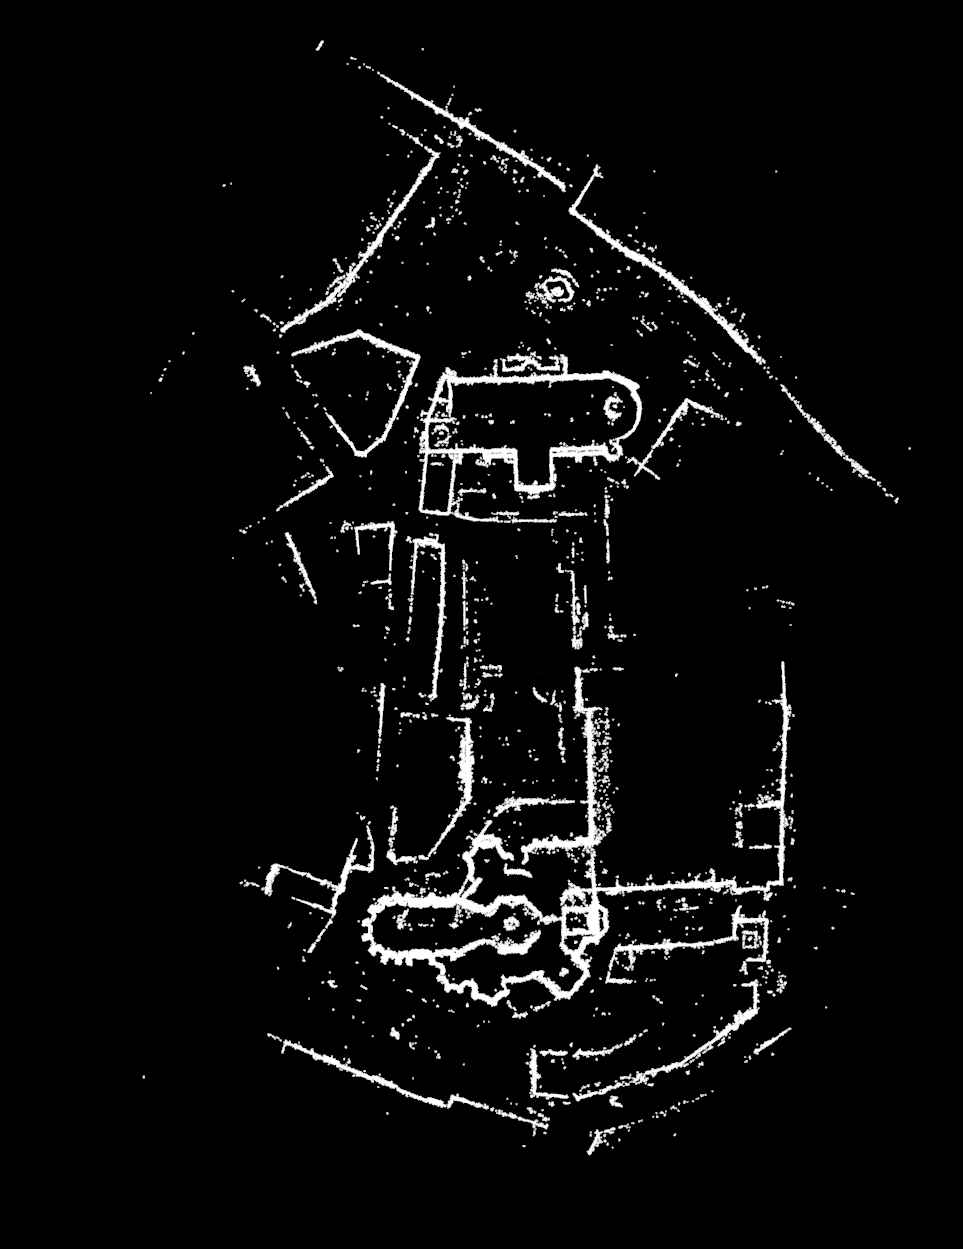
\includegraphics[width=.8\linewidth]{images/Selection_031.png}
  \caption{Original input}
  \label{fig:sfig1}
\end{subfigure}%
\begin{subfigure}{.5\linewidth}
  \centering
  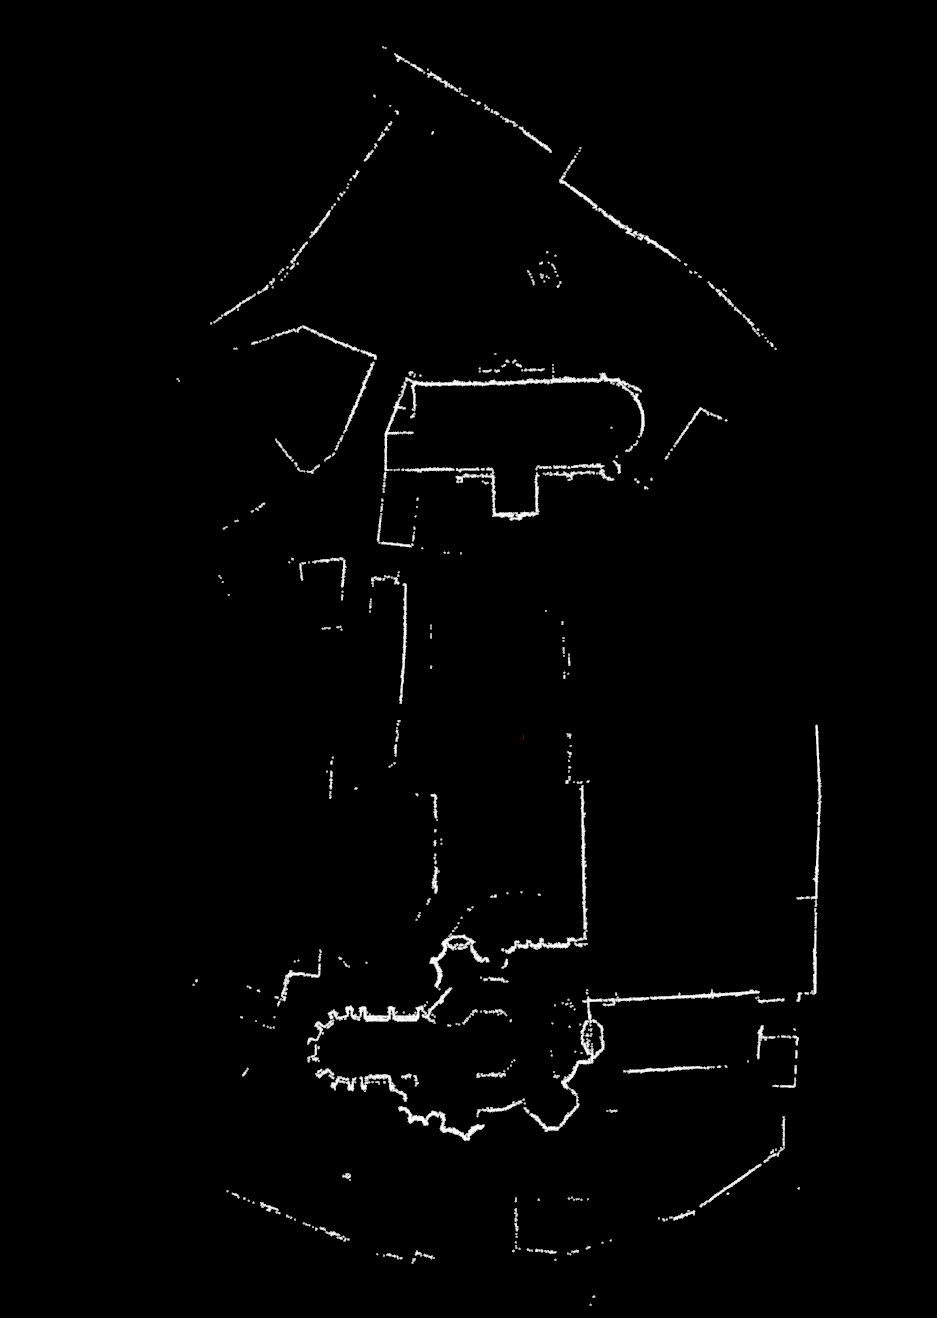
\includegraphics[width=.8\linewidth]{images/Selection_032.png}
  \caption{Output after filter}
  \label{fig:sfig2}
\end{subfigure}

\end{figure}


To further reduce the amount of noise, we implemented a filtering chain, consisting of 

\begin{itemize}
   \item Any given point needs at least 50 neighbors in a radius of 2 meters to be considered a valid measurement
   \item Statistical outliers are removed with a mean of 8 and a standard deviation of 1. This further removes outliers
   \item Only 1/8 of all remaining points are randomly chosen to reduce the computational load
\end{itemize}

\subsection{Initial alignment}

\begin{figure}
\begin{subfigure}{.5\linewidth}
  \centering
  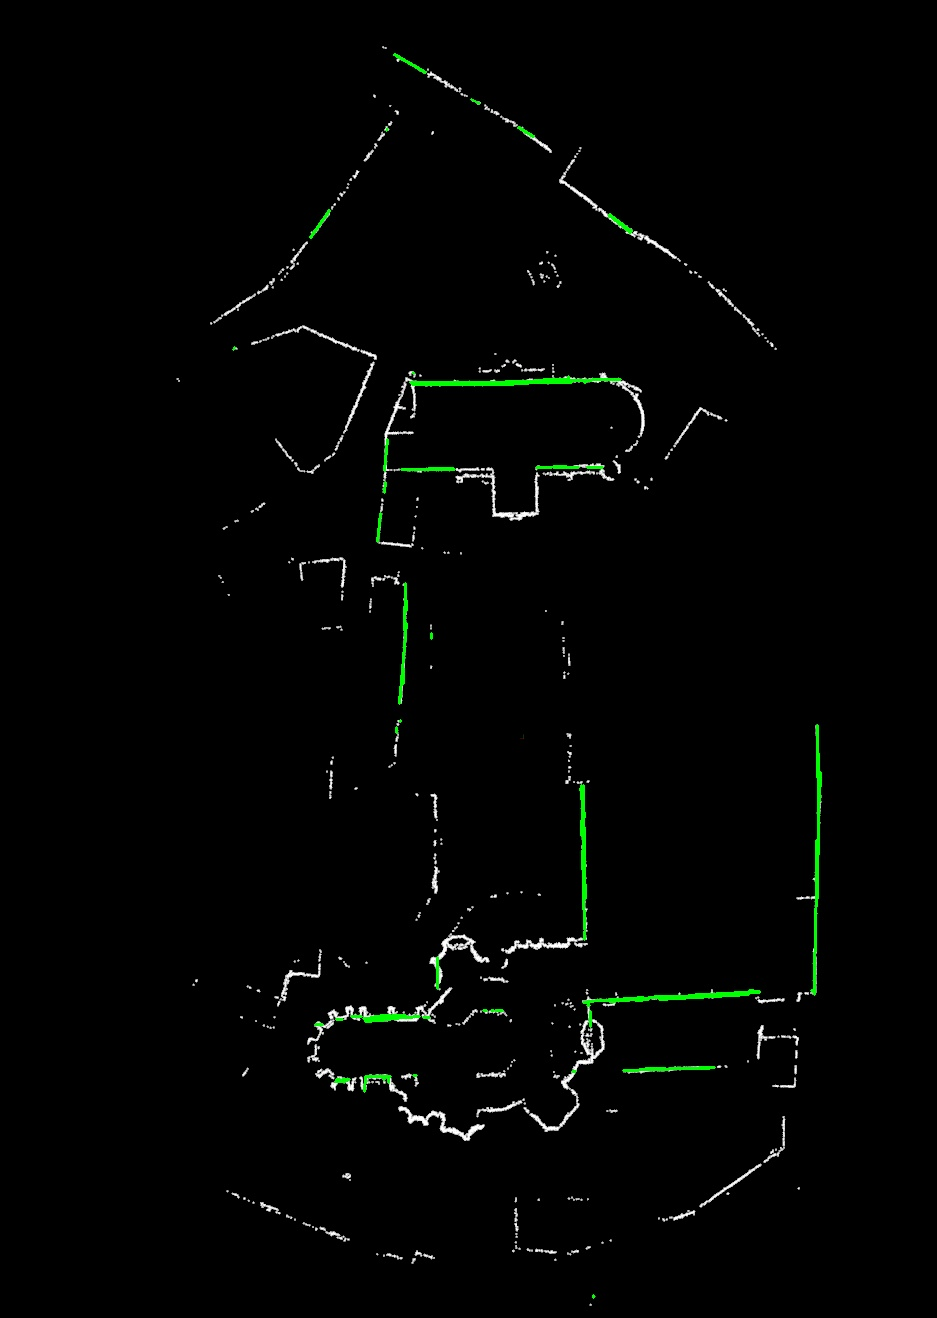
\includegraphics[width=.8\linewidth]{images/houghlines6.jpg}
  \caption{Hough corner detector}
  \label{fig:hough}
\end{subfigure}%
\begin{subfigure}{.5\linewidth}
  \centering
  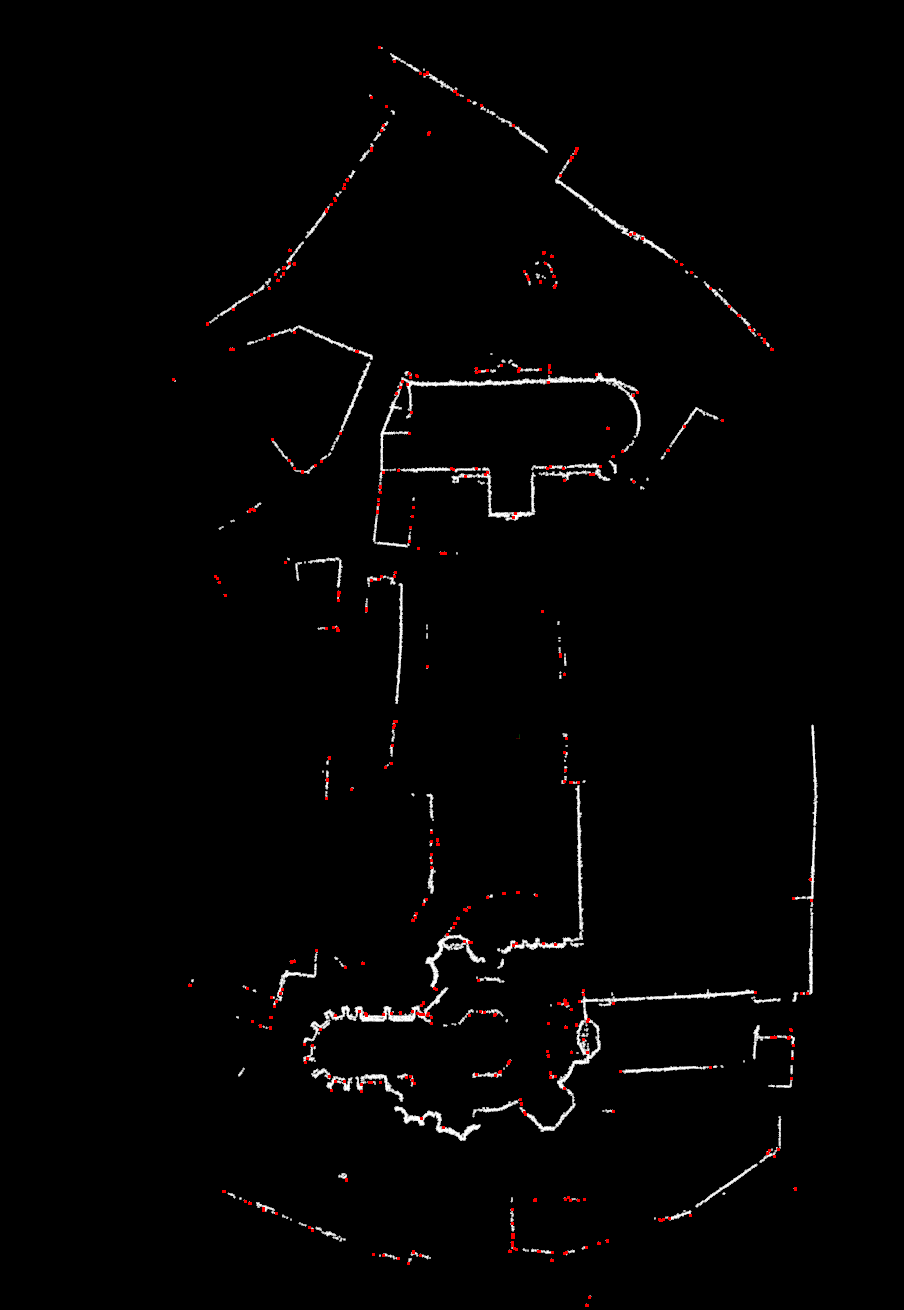
\includegraphics[width=.8\linewidth]{images/harris.png}
  \caption{Harris corner detector}
  \label{fig:harris}
\end{subfigure}
\\
\begin{subfigure}{1\linewidth}
  \centering
  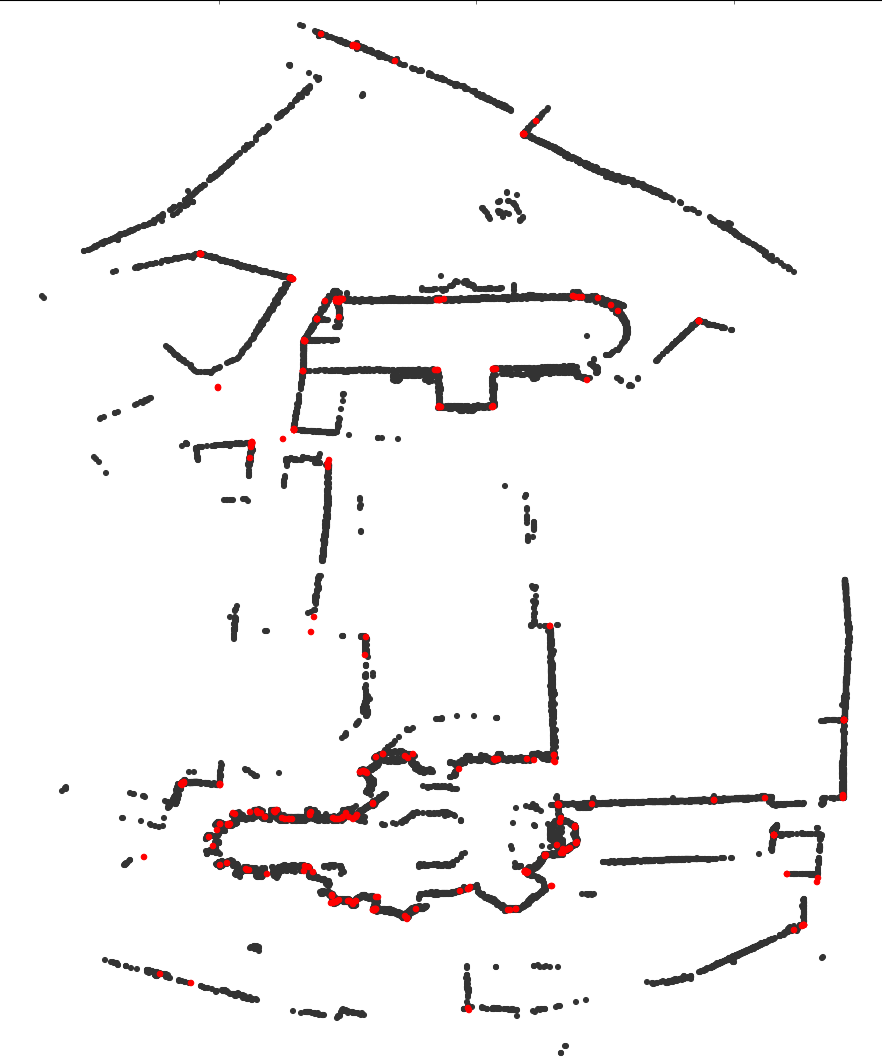
\includegraphics[width=.8\linewidth]{images/ransac_corner.png}
  \caption{RANSAC based corner detection}
  \label{fig:ransac_corner}
\end{subfigure}

\end{figure}

As stated before, the initial alignment of the two pointclouds is crucial for successful ICP matching. 
In order to find a good initial alignment, we try to find corner points in the measured data. 

There exist a number of corner detectors that are well researched. Some of the most notable ones, the Hough-transform~\cite{illingworth1988survey} and the Harris-detector~\cite{harris1988combined} were tried, but didn't deliver sufficient results. The properties of our data are also not extremely well suited for these algorithms which were primarily developed for images. 

We developed an approach based on the Random Sample Consensus algorithm (RANSAC)~\cite{fischler1981random}. RANSAC is able to detect lines in a robust way. Our process looks like this:

\begin{itemize}
    \item Choose random point from point cloud
    \item Select nearest n neighbors from kd-tree and insert into sub point cloud
    \item Find best line with RANSAC
    \item Remove all inliers from sub point cloud
    \item If more than threshold points remaining, find second best line by running RANSAC again
    \item Check angle between both lines (if angle to small or wide, reject)\footnote{Rejecting intersection points based on angle is possible for us since we are primarily interested in corners that meet at about 90 degree. This is due to the fact that we are working with city scapes.} 
    \item If line is found, calculate intersection point
    % \item Reject if intersection point is not close to points in sub point cloud
\end{itemize} 

After a certain, arbitrary numbers of corners is found, we use the map of corners to match the OpenStreetMap data. Therefore we randomly select 3 points from the corner map, and calculate a corresponding transformation to three randomly selected points on the OSM data. This makes it possible to calculate an error and improve or reject several initial transformations.

We then choose the best transformation and use it as initial transformation for the ICP.

\begin{figure}
  \centering
  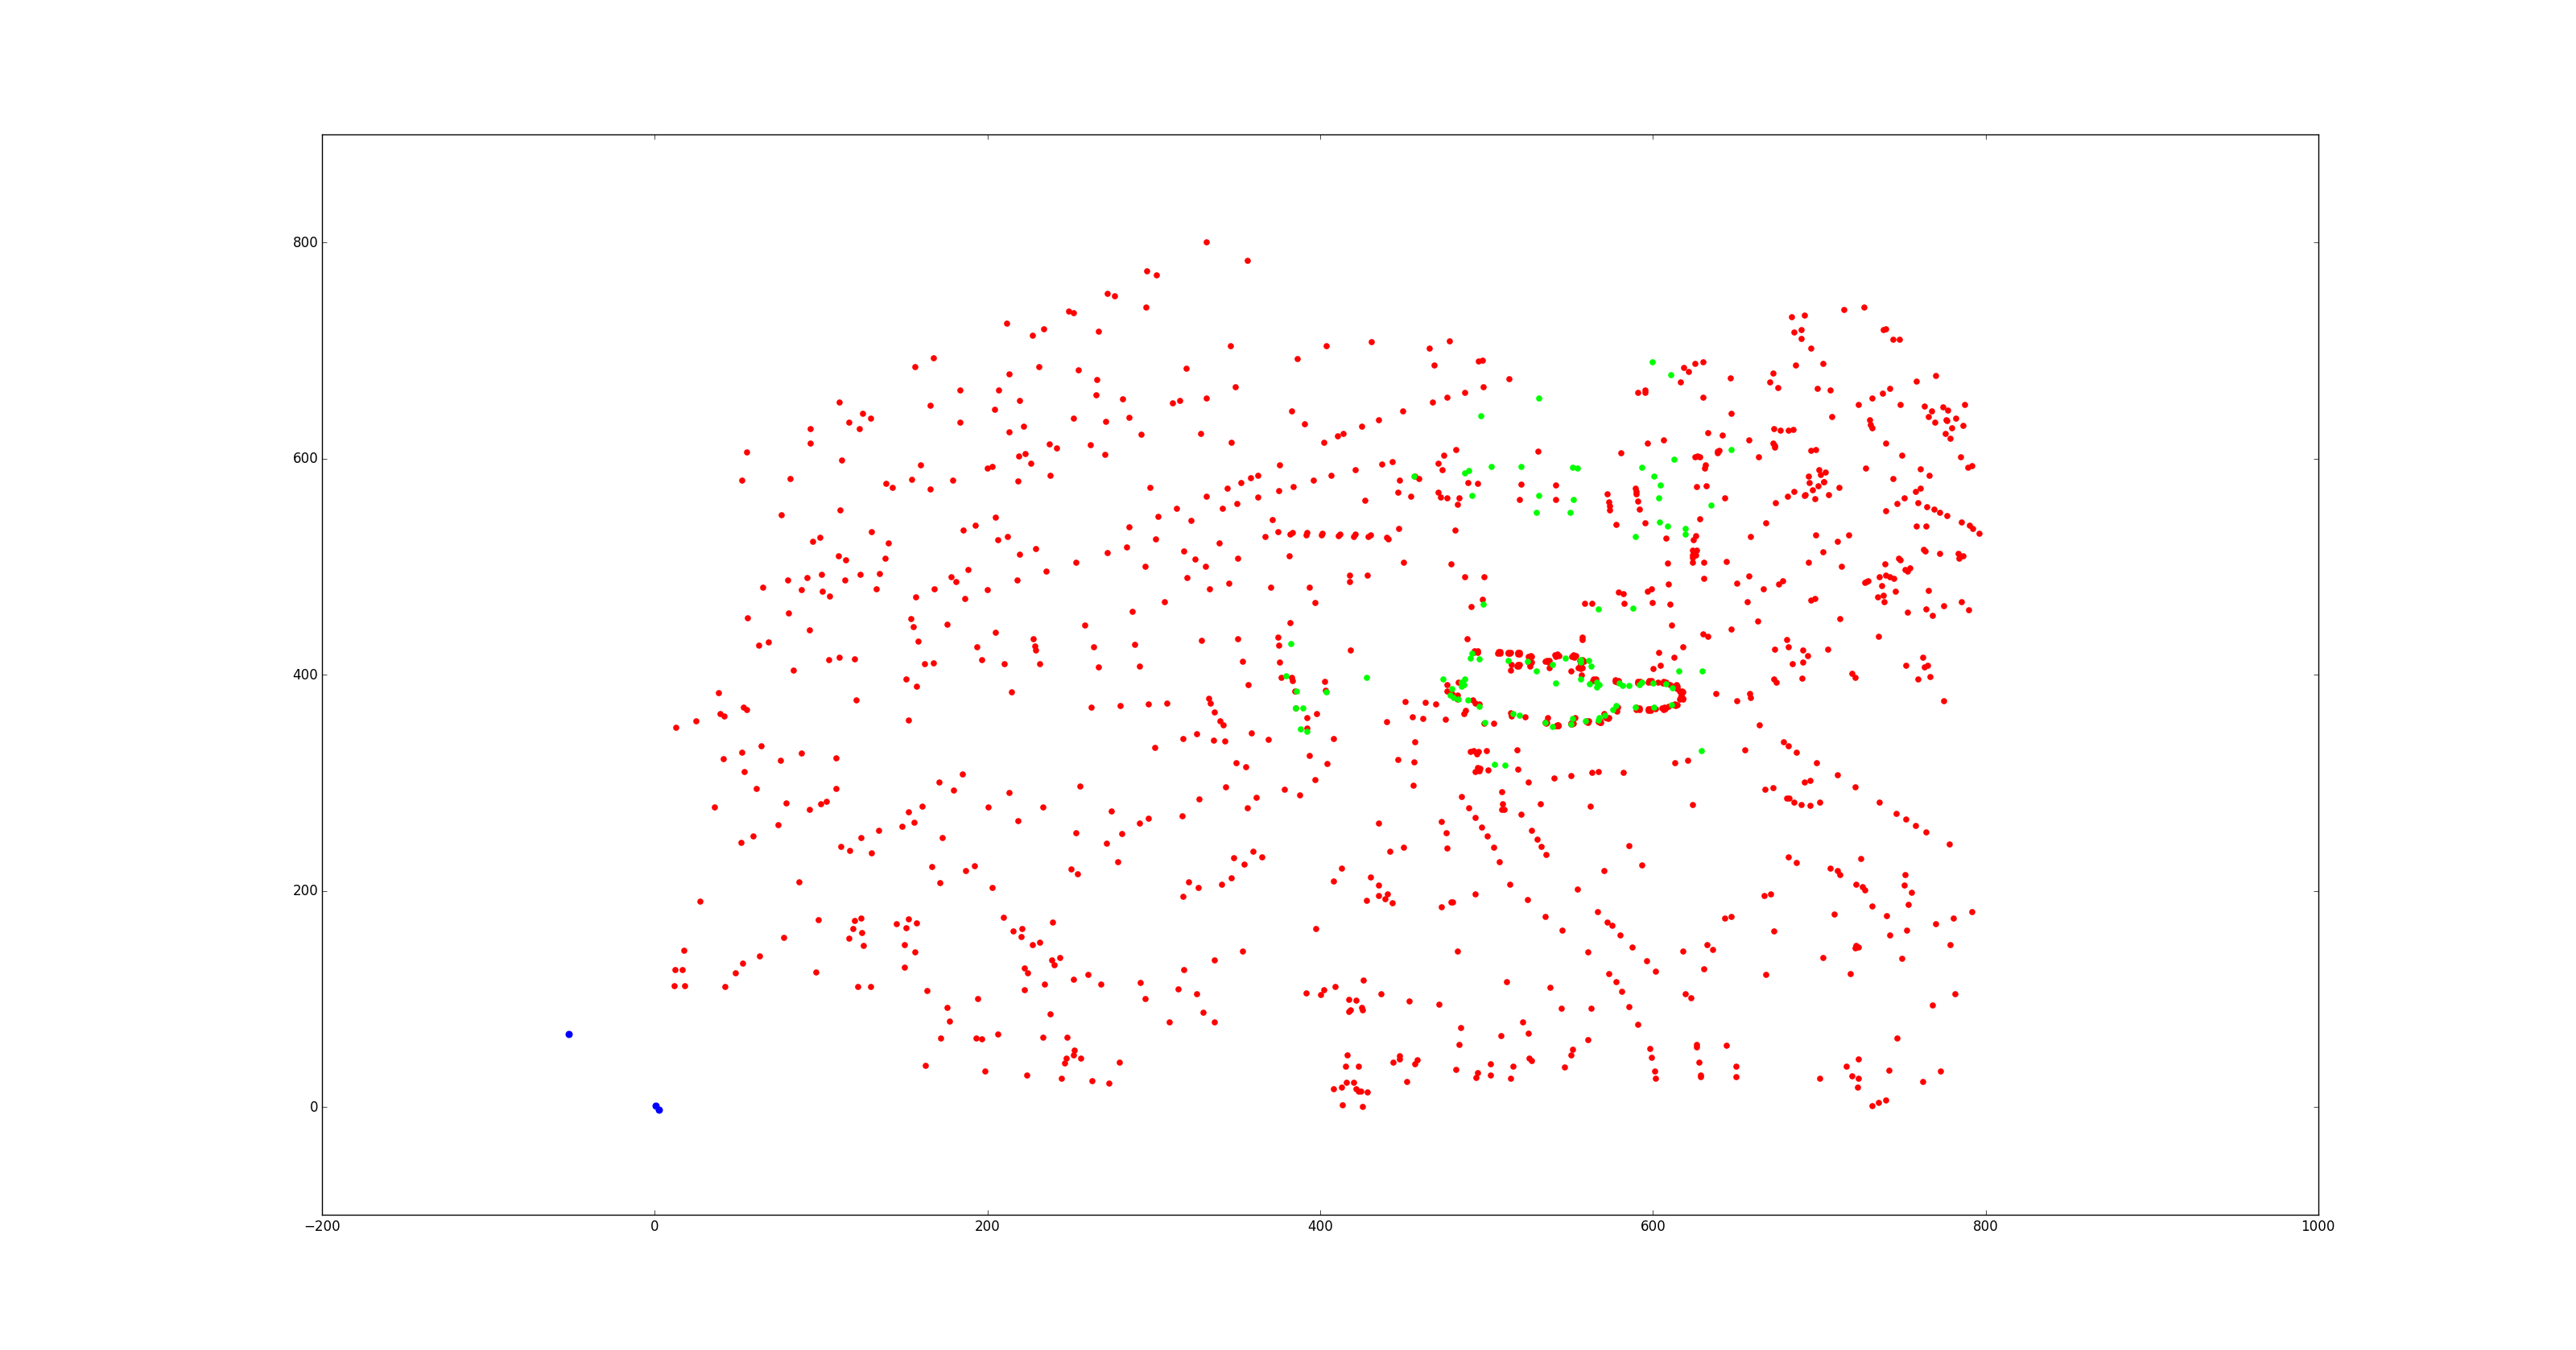
\includegraphics[width=.8\linewidth]{images/goodmatch.png}
  \caption{Fitted after 5000000 iterations}
  \label{fig:goodmatch}
\end{figure}

\section{Conclusion}

\begin{figure}

  \centering
  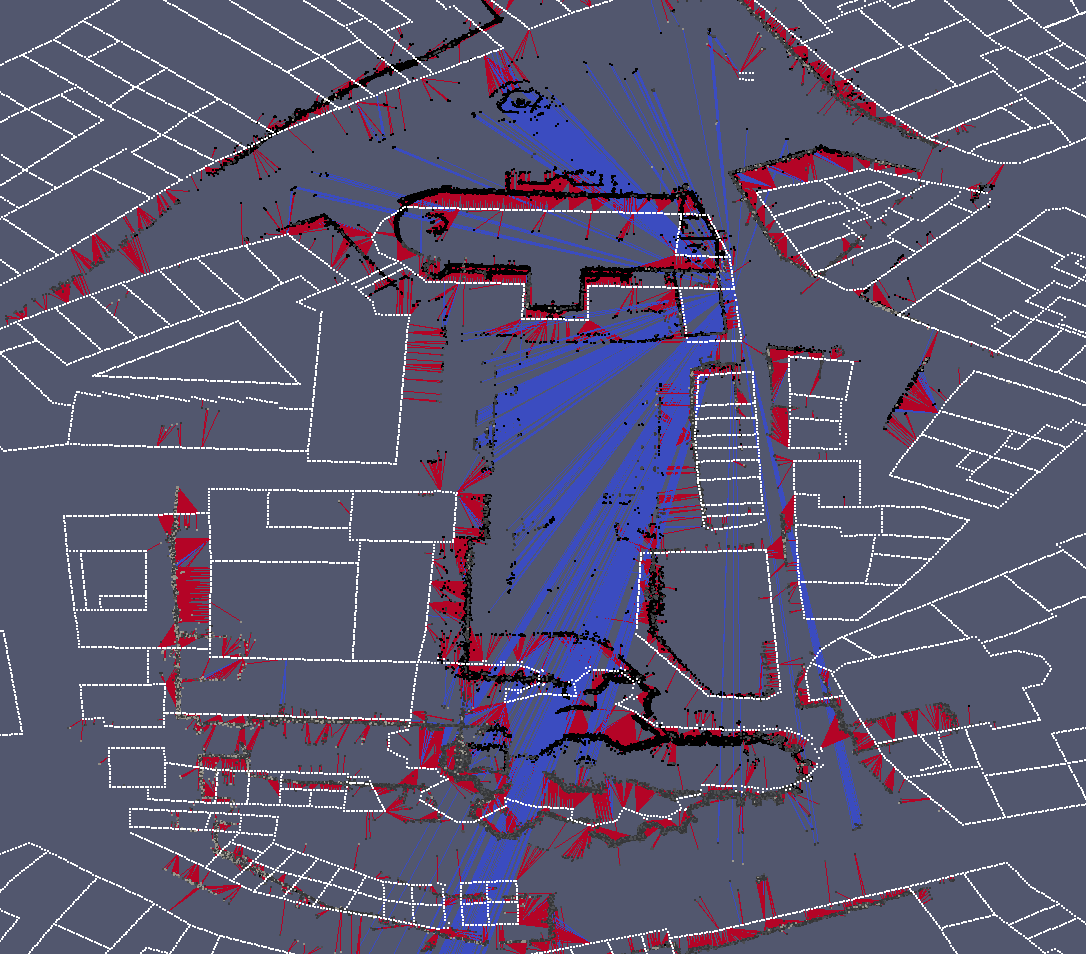
\includegraphics[width=.8\linewidth]{images/result_icp.png}
  \caption{Result from ICP\\Blue lines are considered outliers by algorithm, and red lines indicate matched neighbor}
  \label{fig:icpresult}

\end{figure}

The normal estimation and subsequent filtering provided data that was very well suitable for fitting to underlying building outline data. 
What proved a problem is that ICP implementations usually do not respect scaling or shearing as issue. The corner matching approach we implemented would theoretically work well, however, due to the scale of the problem the brute force approach we implemented was too inefficient to find a good match in reasonable time. 

As expected the ICP, initialized with an approximate translation and rotation as well as prescaled worked well (cf. Figure \ref{fig:icpresult}).

\section{Further ideas}

Feature matching is not an untackled problem as it is used for other problems such as image correspondence analysis based on e.g. scale invariant features as well. Instead of relying on a brute force search with random points, which is very unlikely to yield good results, we should have invested more time to find a more intelligent way of matching features (corners) from the two point clouds.

A simple idea to make the search faster would be to consider only local features for the translation. Instead of randonmly select features from the whole pointcloud, the corners should be spatially close to each other (for example select a combination of three points from the 5 nearest neighbors to a random point). In the same way the features should be selected from the reference cloud. This could easily increase the search speed in a meaningful amount.

We had some ideas to extend the ICP algorithm to also include a term for the scale. Since the SVD decomposition also contains a middle ($\Sigma$) term, that can be interpreted as scaling transformation, we thought we could use this for our result.
However, given the limited time frame we did not succeed in implementing this extension in \texttt{libpointmatcher}.


{\small
\bibliographystyle{ieee}
\bibliography{egbib}
}


\end{document}
